% Page 071 — page imprimée 67
% La famille Roussel du Villaret au Château d’Ayres (suite)

C’est en 1914 que naquit leur unique fille Geneviève dite Ginette. Hélène et Jules Roussel
passaient l’hiver à Paris en compagnie de leur famille car Hélène avait une sœur prénommée
Blanche que tout le monde appelait Annie, et un frère Frédéric dont elle était très proche.
Ginette poursuivit ses études et fut embauchée par Hermès.

\medskip

\textbf{La période 1939-1945 : années de guerre}

\medskip

A la déclaration de guerre en Août 1939 de nombreuses familles en vacances à Meyrueis y
restèrent par peur des bombardements : les souvenirs de la guerre de 1914 étaient encore très
vifs. Des Parisiens et des Marseillais ou des Lyonnais, comme nous, bientôt suivis par des
familles du Nord ou d’Alsace passèrent l’automne puis l’hiver à Meyrueis. Les maris étaient
mobilisés ou continuaient à travailler en ville. Après l’armistice, des étrangers souvent
espagnols, des insoumis, des juifs qui sentaient venir le temps des rafles et des déportations,
après les lois édictées par l’administration pétainiste se cachèrent dans des villages et les écarts
et un certain nombre restèrent au château d’Ayres qui ensuite fut occupé par l’Etat Major des
Chantiers de Jeunesse. Certains de ces jeunes, étrangers ou juifs, purent,de Meyrueis,gagner
l’Espagne.

\medskip

En effet l’armée française avait été supprimée mais il restait un service plus ou moins civil
avec un bel uniforme vert ainsi que le béret des chasseurs alpins. C’était les « Chantiers de
Jeunesse * ». Des centaines de jeunes furent embauchés pour divers travaux à la campagne.
A Meyrueis ils étaient dispersés dans plusieurs unités abattant des arbres et faisant du charbon
de bois pour les gazogènes : (moteur fonctionnant au charbon de bois remplaçant dans les
voitures les moteurs à explosion et à essence). On en trouvait à Rousses et à la Pépinière sur le
Bétuzon, aux Oubrets ou à Valbelle sur la Brèze etc…

\medskip

* voir plus loin l’Histoire des Chantiers.

\begin{center}
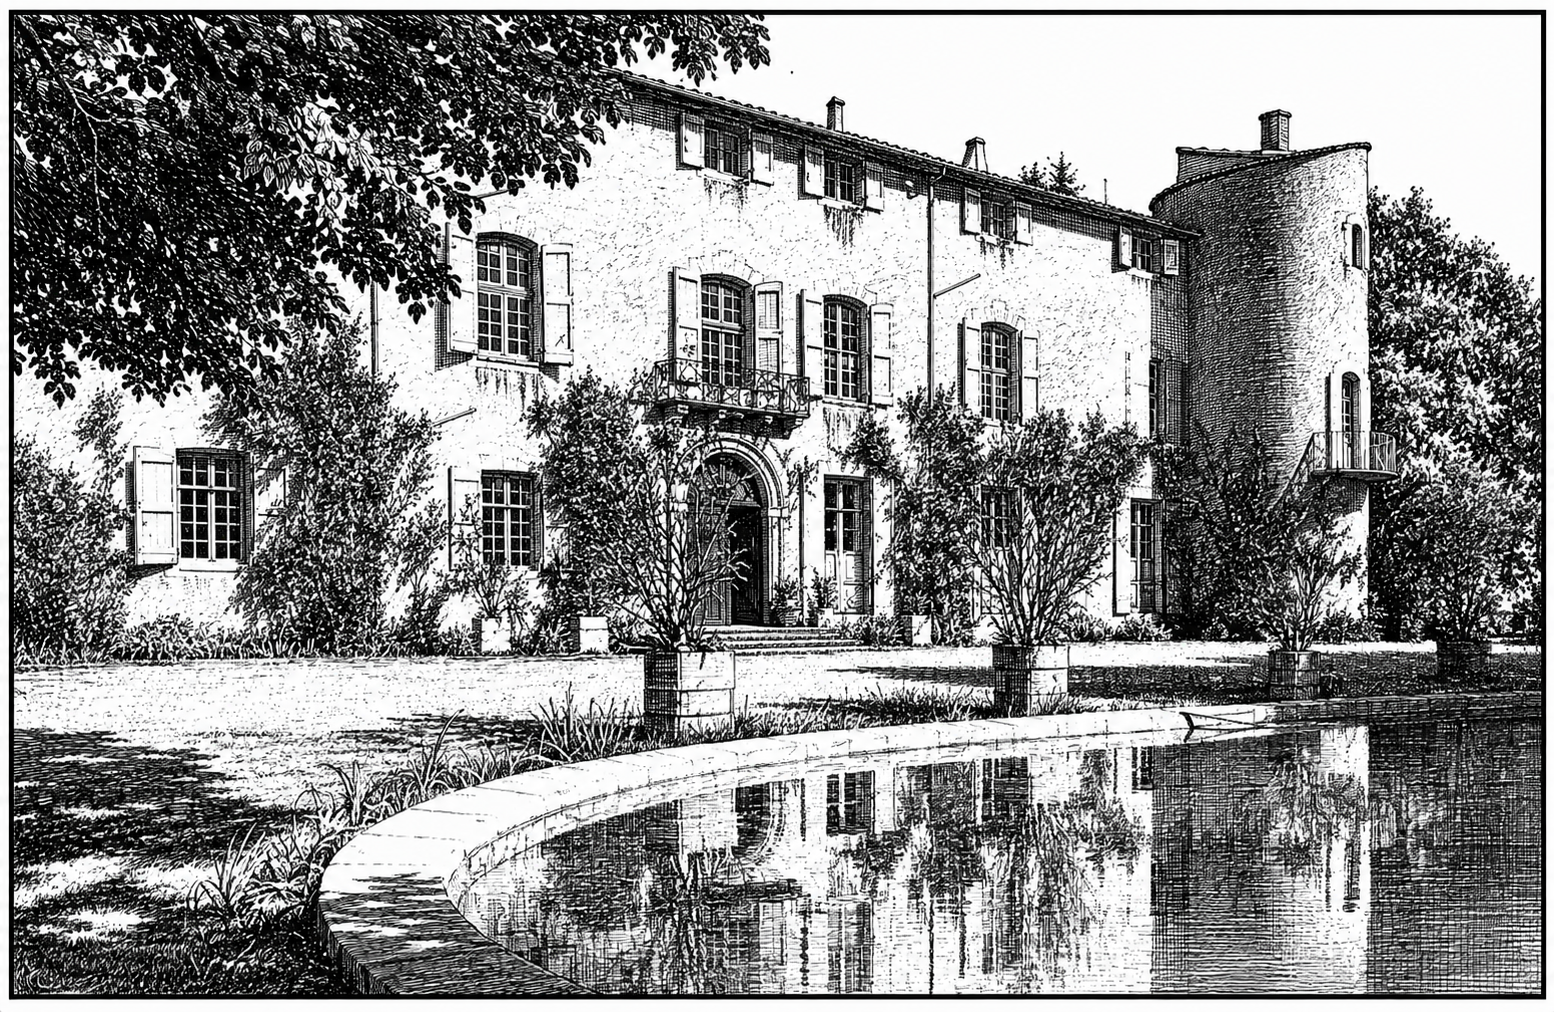
\includegraphics[width=0.78\textwidth]{imgs/071}
\end{center}
